\begin{frame}{MANV}
	\begin{itemize}
		\item MANV: \alert{Massenanfall von Verletzten}
		\item Begriff aus dem Rettungswesen
		\item Tritt ein bei einem Ereignis mit vielen Verletzten
		\item Probleme:
		      \begin{itemize}
			      \item Koordination der Rettungskräfte
			      \item Verteilung von Ressourcen
			      \item Außergewöhnliche Situation auch für Rettungskräfte
		      \end{itemize}
	\end{itemize}
\end{frame}

\begin{frame}{MANV - Beispiele}
	\begin{examples}
		\begin{figure}
			\begin{center}
				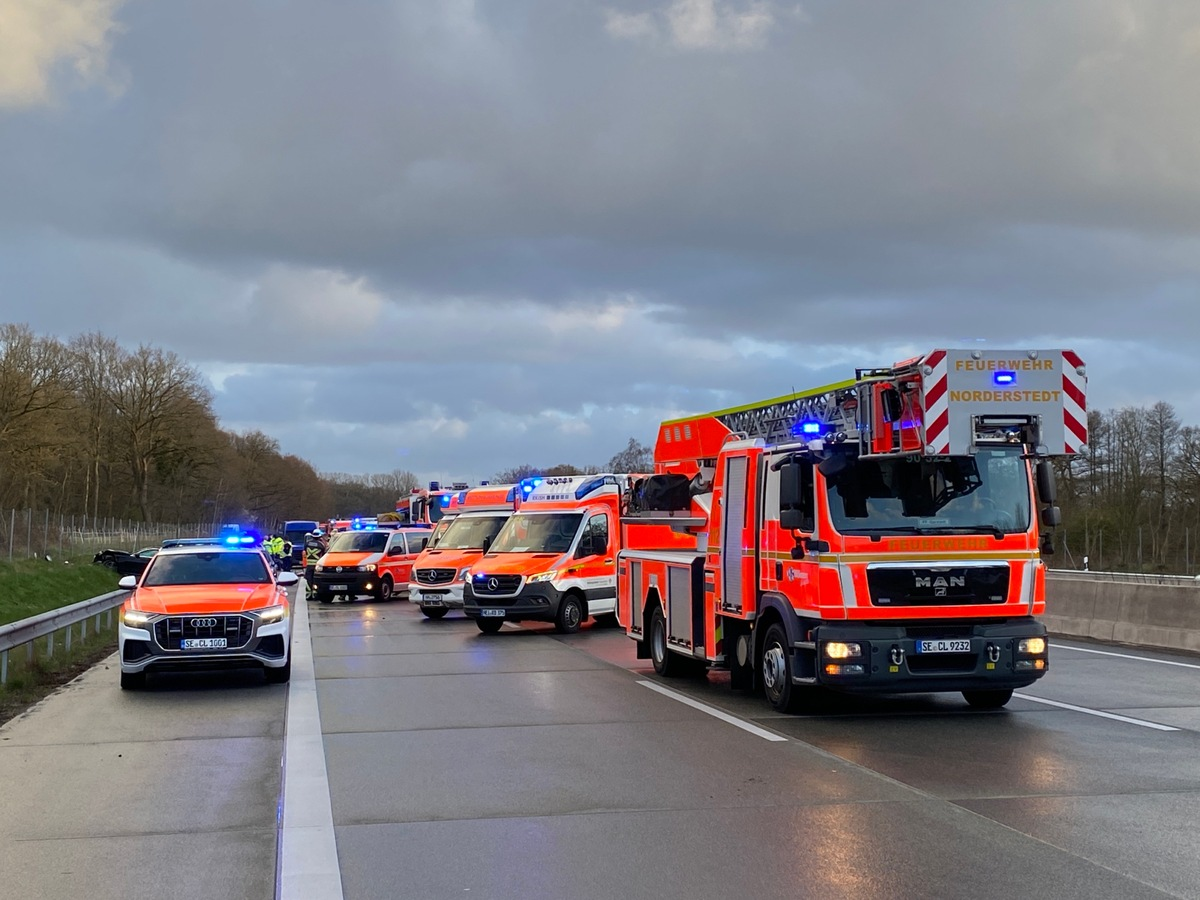
\includegraphics[width=0.4\textwidth]{images/autounfall.jpg}
			\end{center}
			\caption{Autounfall auf A7 mit 11 Betroffenen, davon einer tödlich verletzt.\cite{manv-a7}}\label{fig:autounfall}
		\end{figure}
	\end{examples}
\end{frame}

\begin{frame}{MANV - Beispiele}
	\begin{examples}
		\begin{figure}
			\begin{center}
				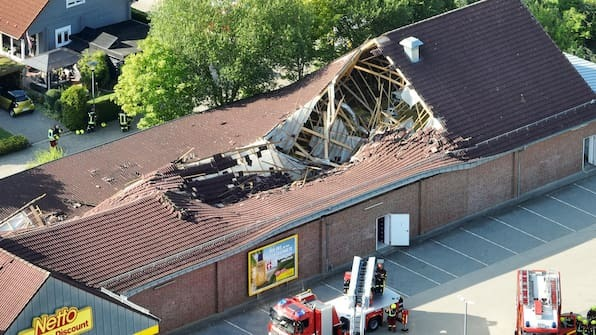
\includegraphics[width=0.5\textwidth]{images/ratzeburg-netto.jpg}
			\end{center}
			\caption{Dacheinsturz eines Supermarktes in Ratzeburg. 12 Leichtverletzte.\cite{manv-ratzeburg}}\label{fig:netto}
		\end{figure}
	\end{examples}
\end{frame}

\begin{frame}
	\begin{examples}
		\begin{figure}
			\begin{center}
				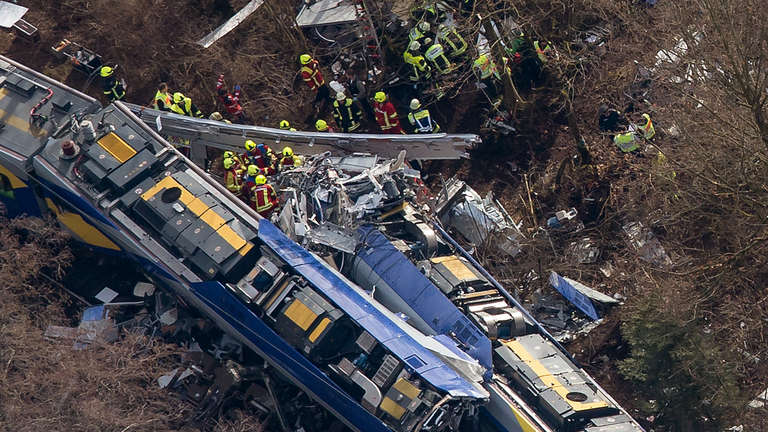
\includegraphics[width=0.5\textwidth]{images/bad-aibling.jpg}
			\end{center}
			\caption{Zugunglück von Bad Aibling. 12 Tote, 18 Schwerverletzte, 63 Leichtverletzte.\cite{manv-badaibling}}\label{fig:badaibling}
		\end{figure}
	\end{examples}
\end{frame}
